\section{Associating clock time and calendar date}
\label{sec-change-location}

\textbf{Created by:} Arkopaul Sarkar \\
\textbf{Modified by:} Arkopaul Sarkar \\

\subsection*{Scenario Objective}

This scenario illustrates how to associate clock time and calendar dates with the instances of time. While the ability to store the clock time and calendar date lets the users perform various quantitative analyses on the processes and their durations, a wide variety of clock and calendar systems makes it challenging to represent the date and times in the correct format. We include use cases depicting basic to advanced methods of representing date and time values of the temporal instances.


\subsection*{General Pattern Description}

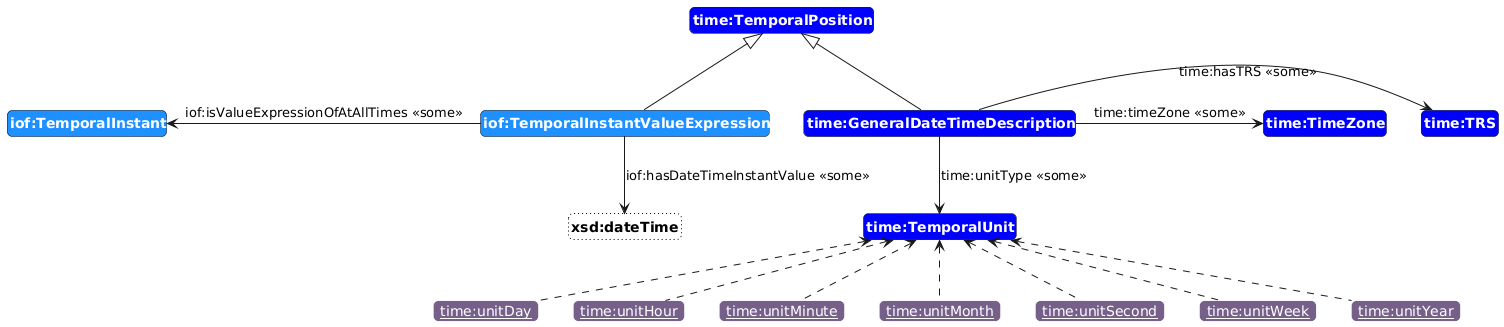
\includegraphics[scale=0.28]{scenarios/clock-time-calendar-date/images/general-clock-calendar.png}

\subsubsection*{Use Case: Launch of first iPhone} 
The original iPhone was first launched on June 29, 2007 during the Macworld Conference \& Expo in San Francisco, California. In the following three patterns, the date and time of the launch are captured in 1) XSD dateTime format, 2) in a specific time zone, and 3) using a custom date and time format. The process \texttt{launch-of-iphone} is not detailed further except the temporal interval it occupies. This instance of temporal interval is then connected to its first temporal instant, for which the calendar date and clock time are assigned.   

\subsubsection*{Use-Case Pattern Description}

\paragraph{XSD dateTime format \\}

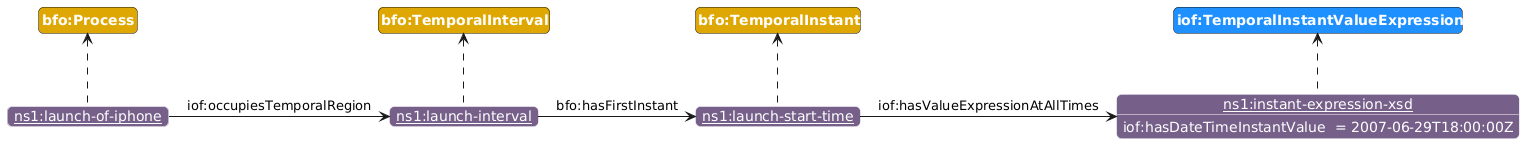
\includegraphics[scale=0.29]{scenarios/clock-time-calendar-date/images/uc1-xsd.png}

The above pattern shows that the IOF Core data property \texttt{hasDateTimeInstantValue} can associate the date and time value in \texttt{xsd:dateTime} format. If the date and time values can be expressed in XSD format, this pattern does not require any reference to OWL Time ontology. Also, \texttt{xsd:dateTime} format already has provision for mentioning time zone (e.g., 2007-06-29T18:00:00-05:00 for a UTC-5 timezone). However, as XSD:dateTime datatype is the range of \texttt{hasDateTimeInstantValue}, no other XSD type or a different format can be expressed using this pattern. 

\paragraph{Custom date and time format \\}



\subsubsection*{Data Mapping Description}

\begin{verbatim}
INSERT DATA {
    ns1:launch-of-iphone a bfo:Process;
                         bfo:occupiesTemporalRegion ns1:launch-interval;
    ns1:launch-interval a bfo:TemporalInterval;
                        iof:hasFirstInstant ns1:launch-start-time.
    ns1:launch-start-time a bfo:TemporalInstant;
                        iof:hasValueExpressionAtAllTimes ns1:instant-expression-xsd.
    ns1:instant-expression-xsd a iof:TemporalInstantValueExpression; 
                        iof:hasDateTimeInstantValue 2007-06-29T18:00:00Z^^xsd:dateTime.
}
\end{verbatim}


\subsubsection*{Data Validation}

